\documentclass[letter,10pt,notitlepage]{article}
\usepackage[utf8x]{inputenc}
\usepackage{fullpage}
\usepackage{subfigure}
\usepackage[pdftex]{graphicx}
\usepackage{amsmath,amssymb,mathtools}
\usepackage{cancel}
\usepackage{rotating}
\usepackage{verbatim}
%\usepackage{natbib}
\newcommand*{\oline}[1]{\overline{#1\mathstrut}}
%opening
%\title{}
%\author{}
%\maketitle

\begin{document}
\section*{Definitions}
\begin{minipage}[t!]{80mm}
\begin{itemize}
\item $U_1$, streamwise mean velocity ($U_2=U_3=0$).
\item $u_1,u_2,u_3$, are the fluctuating velocities along x, y, z, coordinates respectively
\item $\nu$, kinematic viscosity
\item Homogeneous along x and z direction, i.e., $\partial_x \oline{(\cdot)}=\partial_z \oline{(\cdot)}=0$
\end{itemize}
\end{minipage}
\hfill
\begin{minipage}[t!]{90mm}
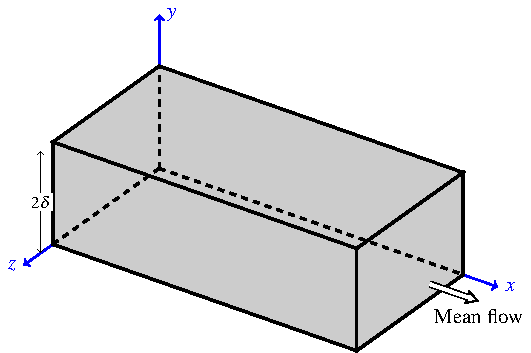
\includegraphics[angle=0.0,width=\textwidth]{channelFig.pdf}
\end{minipage}

\section*{Statistical moments and their budgets}
The second-, third- and fourth-order moments of the Navier-Stokes equations for the case of parallel flow
are given in Equations~\eqref{eqn:2mom}, \eqref{eqn:3mom} and \eqref{eqn:4mom}, respectively.  The terms written on the right-hand-side 
balance the total derivative.  For parallel-flows the spatial gradient in the convective term is zero.  
Furthermore, with a constant streamwise pressure gradient, the temporal derivative is zero.  
Hence in the unstrained fully-developed channel flow, $D_t=0$.  Due to straining the material derivative is $\mathcal{D}_t=\partial_t \neq 0$.  The applied strain causes the moments to evolve in time, anologous to spatial development of an adverse pressure gradient boundary layer.  In otherwords, spatial derivative is replaced by a time derivative.


%\noindent
\begin{flalign}
 &&\partial_t\overline{u_iu_j} &= \mathcal{P}_{ij}^S+\mathcal{P}_{ij}^A+\mathcal{T}_{ij}+\Pi_{ij}+\varepsilon_{ij}+\mathcal{D}_{ij} &&\label{eqn:2mom}\\
&\text{where} \hidewidth \nonumber\\
&&\mathcal{P}_{ij}^S &= -\overline{u_iu_2}\partial_2U_j-\overline{u_ju_2}\partial_2U_i &&\nonumber\\
&&\mathcal{P}_{ij}^A &= -\overline{u_iu_k}A_{jk}-\overline{u_ju_k}A_{ik} &&\nonumber\\
&&\mathcal{T}_{ij} &= -\partial_2\overline{u_2u_iu_j} &&\nonumber\\
&&\Pi_{ij} &= -(1/\rho) (\overline{u_j\partial_ip}+\overline{u_i\partial_jp}) &&\nonumber\\
&& \varepsilon_{ij} &= -2\nu \overline{\partial_ku_i\partial_ku_j} &&\nonumber\\
&& \mathcal{D}_{ij} &= \nu \partial_2^2 \overline{u_iu_j} &&\nonumber
\end{flalign}
%\noindent
\begin{flalign}
&&\partial_t\overline{u_iu_ju_l} &= 
   \mathcal{P}_{ijl}^S+\mathcal{P}_{ijl}^A+\mathcal{P}_{ijl}^T+\mathcal{T}_{ijl}+\Pi_{ijl}
   +\varepsilon_{ijl}+\mathcal{D}_{ijl} &&\label{eqn:3mom}\\
&\text{where} \hidewidth \nonumber\\
%\text{where} ~~~~~~~~~~~~~~~~~~~~~~~~~~~~~~~~&\\
&&\mathcal{P}_{ijl}^S &= -\overline{u_iu_ju_2}\partial_2U_l-\overline{u_ju_lu_2}\partial_2U_i-\overline{u_lu_iu_2}\partial_2U_j &&\nonumber \\
&&\mathcal{P}_{ijl}^A &= -\overline{u_iu_ju_k}A_{lk}-\overline{u_ju_lu_k}A_{ik}-\overline{u_lu_iu_k}A_{jk} &&\nonumber\\
&&\mathcal{P}_{ijl}^T &= \overline{u_iu_j}\partial_2\overline{u_2u_l}+\overline{u_ju_l}\partial_2\overline{u_2u_i}+\overline{u_lu_i}\partial_2\overline{u_2u_j} &&\nonumber \\
&&\mathcal{T}_{ijl} &= -\partial_2\overline{u_2u_iu_ju_l} &&\nonumber \\
&&\Pi_{ijl} &= -(1/\rho) (\overline{u_iu_j\partial_lp}+\overline{u_ju_l\partial_ip}+\overline{u_lu_i\partial_jp}) &&\nonumber \\
&&\varepsilon_{ijl} &= -2\nu (\overline{u_i\partial_ku_j\partial_ku_l}+\overline{u_j\partial_ku_i\partial_ku_l}+\overline{u_l\partial_ku_i\partial_ku_j}) &&\nonumber\\
&&\mathcal{D}_{ijl} &= \nu\partial_2^2\overline{u_iu_ju_l} &&\nonumber
\end{flalign}
%\noindent
\begin{flalign}
&&\partial_t\overline{u_iu_ju_lu_m} &= 
%&&&\partial_t\overline{u_iu_ju_lu_m}+U_2\partial_2\overline{u_iu_ju_lu_m} = 
\mathcal{P}_{ijlm}^S+\mathcal{P}_{ijlm}^A+\mathcal{P}_{ijlm}^T+\mathcal{T}_{ijlm}+\Pi_{ijlm}
+\varepsilon_{ijlm}+\mathcal{D}_{ijlm} &&\label{eqn:4mom}\\
&\text{where} \hidewidth \nonumber\\
&&\mathcal{P}_{ijlm}^S &= -\overline{u_iu_ju_lu_2}\partial_2U_m-\overline{u_ju_lu_mu_2}\partial_2U_i-\overline{u_lu_mu_iu_2}\partial_2U_j-\overline{u_mu_iu_ju_2}\partial_2U_l &&\nonumber\\ 
&&\mathcal{P}_{ijlm}^A &= -\overline{u_iu_ju_lu_k}A_{mk}-\overline{u_ju_lu_mu_k}A_{ik}-\overline{u_lu_mu_iu_k}A_{jk}-\overline{u_mu_iu_ju_k}A_{lk} &&\nonumber\\
&&\mathcal{P}_{ijlm}^T &= \overline{u_iu_ju_l}\partial_2\overline{u_2u_m}+\overline{u_ju_lu_m}\partial_2\overline{u_2u_i}+\overline{u_lu_mu_i}\partial_2\overline{u_2u_j}+\overline{u_mu_iu_j}\partial_2\overline{u_2u_l} &&\nonumber \\
&&\mathcal{T}_{ijlm} &= -\partial_2\overline{u_2u_iu_ju_lu_m} &&\nonumber\\
&&\Pi_{ijlm} &= -(1/\rho) (\overline{u_iu_ju_l\partial_mp}+\overline{u_ju_lu_m\partial_ip}+\overline{u_lu_mu_i\partial_jp}+\overline{u_mu_iu_j\partial_lp}) &&\nonumber\\
&&\varepsilon_{ijlm} &= -2\nu ( \overline{u_iu_j\partial_ku_l\partial_ku_m}+\overline{u_iu_l\partial_ku_j\partial_ku_m}+\overline{u_ju_l\partial_ku_i\partial_ku_m} &&\nonumber\\
&&& ~~~~~~+\overline{u_ju_m\partial_ku_l\partial_ku_i}+\overline{u_lu_m\partial_ku_j\partial_ku_i}+\overline{u_mu_i\partial_ku_l\partial_ku_j} ) &&\nonumber\\
&&\mathcal{D}_{ijlm} &= \nu\partial_2^2\overline{u_iu_ju_l} &&\nonumber
\end{flalign}

In equation \ref{eqn:2mom}-\ref{eqn:4mom}, budgets on the right hand side are termed as production due to shear($\mathcal{P}^S$), production due to Reynolds stress($\mathcal{P}^T$), turbulent diffusion($\mathcal{T}$), velocity-pressure gradient correlation($\Pi$), dissipation($\varepsilon$) and viscous diffusion($\mathcal{D}$).  The applied strain produces source terms in all the moment equations, which is called production due to applied strain ($\mathcal{P}_{ij}^A$).  The terminologies used to describe the budget terms are inherited from second-moment closure, and do not necessarily represent physical behavior (e.g., `production' can be negative and `dissipation' can be positive).

The velocity pressure gradient term is decomposed as $\Pi = \psi + \phi$, where $\psi$ is pressure transport term and $\phi$ the pressure-strain term.  Expressions of the decomposed terms in the second-, third- and fourth-order moment are given below.
\begin{align}
\psi_{ij} &= \frac{-1}{\rho} \left( \partial_2\oline{pu_j}\delta_{2i}+\partial_2\oline{pu_i}\delta_{2j} \right) \\
\phi_{ij} &= \frac{1}{\rho} \left( \oline{p\partial_iu_j}+\oline{p\partial_ju_i} \right) \\
\psi_{ijl} &= \frac{-1}{\rho} \left( \partial_2\oline{pu_iu_j}\delta_{2l}+\partial_2\oline{pu_ju_l}\delta_{2i}+\partial_2\oline{pu_lu_i}\delta_{2j} \right) \\
\phi_{ijl} &= \frac{1}{\rho} \left( \oline{p\partial_lu_iu_j}+\oline{p\partial_iu_ju_l}+\oline{p\partial_ju_lu_i} \right) \\
\psi_{ijlm} &= \frac{-1}{\rho} \left( \partial_2\oline{pu_iu_ju_l}\delta_{2m}+\partial_2\oline{pu_ju_lu_m}\delta_{2i}+\partial_2\oline{pu_lu_mu_i}\delta_{2j}+\partial_2\oline{pu_mu_iu_j}\partial_{2l} \right) \\
\phi_{ijlm} &= \frac{1}{\rho} \left( \oline{p\partial_mu_iu_ju_l}+\oline{p\partial_iu_ju_lu_m}+\oline{p\partial_ju_lu_mu_i}+\oline{p\partial_lu_mu_iu_j} \right)
\end{align}

\end{document}
